% The main file for TUM reports

%% Final document
\documentclass[11pt,a4paper,bibtotoc,idxtotoc,headsepline,footsepline,footexclude,BCOR12mm,DIV13]{scrbook}

% KOMA-Optionen:
%  bibtotoc: include bibliography in table of contents
%  idxtotoc: include index in table of contents
%  headsepline: use horizontalline under heading
%  BCOR: binding correcion (Bindungskorrektur) (e.g.: BCOR5mm)
%  DIV: Number of sheet sections (used for layout) (e.g.: DIV12)

% Set here the title, authors and other stuff to be used for the cover

\def\doctype{Bachelorarbeit in Informatik}
\def\title{On the new threats of social engineering exploiting social networks}
\def\titleGer{Neue Bedrohungen bei Sozialen Netzwerken im Bezug auf Social Engineering}
\def\author{Daniel Siegel}
\def\date{August 15, 2009}

% text to appear in the footer
\def\footertext{}

\usepackage{scrpage2}
\pagestyle{scrheadings}
\ifoot[\footertext]{\footertext} % \footertext set in INFO.TEX

\usepackage[utf8]{inputenc}
\usepackage[T1]{fontenc}
\usepackage[ngerman,english]{babel}
\selectlanguage{english}

\usepackage[pdftex]{graphicx}
\graphicspath{{figures/}}

\usepackage{cmbright}

\usepackage{ifthen}
\usepackage{subfigure}
\usepackage{colortbl}
\usepackage{multirow}
\usepackage{url}
\usepackage{color}
\usepackage{makeidx}
\usepackage{float}
\usepackage{rotating}

\usepackage{styles/tumlogo}
\usepackage{styles/shortoverview}
\usepackage{styles/secnum}


\usepackage[pdftex,colorlinks=true,linkcolor=red,citecolor=red,%
anchorcolor=red,urlcolor=red,bookmarks=true,%
bookmarksopen=true,bookmarksopenlevel=0,plainpages=false%
bookmarksnumbered=true,hyperindex=false,pdfstartview=%
]{hyperref}

\hypersetup{%
  pdftitle    = \title,
  pdfsubject  = {Bachelor thesis},
  pdfauthor   = {Daniel Siegel},
  colorlinks  = true,
  linkcolor   = blue,
  urlcolor    = red,
  breaklinks  = true,
}


%% Fancy chapters

% set the bibliography style
\bibliographystyle{styles/bauermaNum}
%\bibliographystyle{alpha}
%\bibliographystyle{plain}

% Disable single lines at the start of a paragraph (Schusterjungen)
% Disable single lines at the end of a paragraph (Hurenkinder)
\clubpenalty = 10000
\widowpenalty = 10000
\displaywidowpenalty = 10000

%% mark text as preliminary
\usepackage[draft,german,scrtime]{prelim2e}

% Commands to be used within the TUM report document

% comment that appears on the border - very practical !!!
\newcommand{\comment}[1]{\marginpar{\raggedright \noindent \footnotesize {\sl #1} }}

% page clearing
\newcommand{\clearemptydoublepage}{%
  \ifthenelse{\boolean{@twoside}}{\newpage{\pagestyle{empty}\cleardoublepage}}%
  {\clearpage}}



%\makeindex
    %% inter line spacing
%\linespread{1.0}

\makeglossary

\begin{document}

  \frontmatter

  % The front cover for the TUM report document.

% correct BCOR - undo at the end !!!
\def\bcorcor{0.15cm}
\addtolength{\hoffset}{\bcorcor}

\thispagestyle{empty}

 \vspace{4cm}
\begin{center}
  \oTUM{4cm}

  \vspace{5mm}     
  \huge FAKULT{\"A}T F{\"U}R INFORMATIK\\ 
  \vspace{0.5cm}
  \large DER TECHNISCHEN UNIVERSIT{\"A}T M{\"U}NCHEN\\
  \vspace{1mm}

\end{center}

\vspace{15mm}
\begin{center}

  {\Large \doctype}
  \vspace{20mm}

  {\huge\bf \title}\\%[3ex]
  \vspace{15mm}

  {\LARGE  \author}
  \vspace{10mm}

  \begin{figure}[h!]
  \centering
   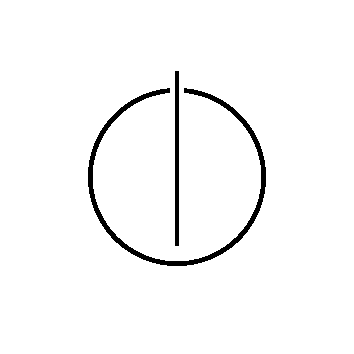
\includegraphics[width=4cm]{styles/informat.png}
  \end{figure}

\end{center}


  \clearemptydoublepage

  % The titlepage for the CAMP report document.

%--------------------------------------------------
% The title page
%--------------------------------------------------

\thispagestyle{empty}

\vspace{10mm}

\begin{center}
  \oTUM{4cm}

  \vspace{5mm}
  \huge FAKULTÄT FÜR INFORMATIK\\
  \vspace{0.5cm}
  \large DER TECHNISCHEN UNIVERSITÄT MÜNCHEN\\
  \vspace{1mm}
\end{center}

\vspace{10mm}
\begin{center}
  {\Large \doctype}
  \vspace{10mm}

  {\LARGE \textbf \title}\\
  \vspace{10mm}

  {\LARGE \textbf \titleGer}\\
  \vspace{10mm}

  \begin{tabular}{ll}
    \Large Author:     & \Large \author \\[2mm]
    \Large Supervisor: & \Large Univ.-Prof. Dr. Claudia Eckert \\[2mm]
    \Large Advisor:    & \Large Dipl.Inf. Werner Streitberger\\[2mm]
    \Large Date:       & \Large August 15, 2009
  \end{tabular}

  \vspace{5mm}

  \begin{figure}[h!]
  \centering
  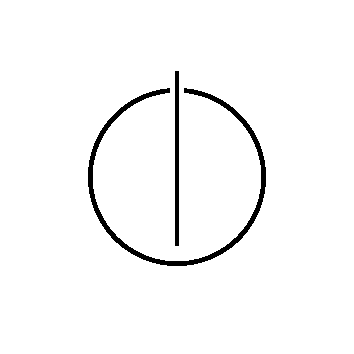
\includegraphics[width=4cm]{styles/informat.png}
  \end{figure}
\end{center}


  \clearemptydoublepage

\thispagestyle{empty}
\selectlanguage{ngerman}
  \vspace*{0.8\textheight}
  \noindent
  Ich versichere, dass ich diese Bachelorarbeit selbstständig verfasst und nur\\
  die angegebenen Quellen und Hilfsmittel verwendet habe.

  \vspace{15mm}
  \noindent
  M{\"u}nchen, den \today \hspace{5cm} \author
\selectlanguage{english}
\newpage


  \clearemptydoublepage
\phantomsection
\addcontentsline{toc}{chapter}{Acknowledgements}	

\vspace*{2cm}

\begin{center}
{\Large \bf Acknowledgments}
\end{center}

\vspace{1cm}

If someone contributed to the thesis... might be good to thank them here.


  % Abstract for the TUM report document
% Included by MAIN.TEX


\clearemptydoublepage
\phantomsection
\addcontentsline{toc}{chapter}{Abstract}	





\vspace*{2cm}
\begin{center}
{\Large \bf Abstract}
\end{center}
\vspace{1cm}

An abstracts abstracts the thesis!

  \tableofcontents

  \clearemptydoublepage

\phantomsection
\addcontentsline{toc}{chapter}{Outline of the Thesis}

\begin{center}
	\huge{Outline of the Thesis}
\end{center}


%--------------------------------------------------------------------
\section*{Part I: Introduction and Theory}

\noindent {\scshape Chapter 1: Introduction}  \vspace{1mm}

\noindent  This chapter presents an overview of the thesis and it purpose. Furthermore, it will discuss the sense of life in a very general approach.  \\

\noindent {\scshape Chapter 2: Theory}  \vspace{1mm}

\noindent  No thesis without theory.   \\

%--------------------------------------------------------------------
\section*{Part II: The Real Work}

\noindent {\scshape Chapter 3: Overview}  \vspace{1mm}

\noindent  This chapter presents the requirements for the process.


  \mainmatter

  \part[Introduction and Theory]{Introduction and Theory}
  \label{part:introAndBackgroundTheory}
  \chapter{Introduction}
\label{chapter:Introduction}



Here starts the thesis with an introduction. Please use nice latex and bibtex entries \cite{latex}. Do not spend time on formating your thesis, but on its content. 
 
\section{Latex Introduction}
There is no need for a latex introduction since there is plenty of literature out there.
 




  \part[The 2nd Part]{The Second Part}
  \label{part:secondP}

  \part*{Appendix}
  \addcontentsline{toc}{part}{Appendix}

  \appendix

  \chapter{Detailed Descriptions}
%\section{Detailed Validation Results}
\label{chapter:DetailedDescriptions}
Here come the details that are not supposed to be in the regular text.

  \clearemptydoublepage

  \bibliography{bibliography/literature}

\end{document}
